\chapter{Towards incorporating sound source information}
\label{ch:mlmann}

% \section*{Abstract}

% \copied{The recent development and deployment of Wireless Acoustic Sensor Networks (WASN) present new ways to address urban acoustic challenges in a smart city context. A focus on improving quality of life forms the core of smart-city design paradigms and cannot be limited to simply measuring objective environmental factors, but should also consider the perceptual, psychological, and health impacts on citizens. This study therefore makes use of short (1 - 2.7s) recordings sourced from a WASN in Milan which were grouped into various environmental sound source types and given an annoyance rating via an online survey with $N=100$ participants. A multilevel psychoacoustic model was found to achieve an overall $R^2=0.64$ which incorporates Sharpness as a fixed effect regardless of the sound source type and Roughness, Impulsiveness, and Tonality as random effects whose coefficients vary depending on the sound source. These results present a promising step torward implementing an on-sensor annoyance model which incorporates psychoacoustic features and sound source type, and is ultimately not dependent on sound level.}

\footnote{The content of this chapter was originally published as \citet{Orga2021Multilevel}, a collaborative work between myself from the SSID team at UCL and Dr Ferran Orga, a researcher at Grup de Recerca en Tecnologies M{\'e}dia, La Salle-URL. Dr Orga and I shared first authorship on this paper. Original data collection was performed by the team at La Salle-URL while the data analysis and modelling strategy was conceived by the team at UCL and implemented by me. Dr Orga and myself drafted the original manuscript, with my work focussing on the analysis method section, results, and discussion of the modelling results.} In \citet{Brown2009acoustic}, the author proposes that one of the underutilised concepts in making use of sound as a resource is the disaggregation of sound sources. He states that `the type of sound sources present is critical in judgements about outdoor sound quality'. The goal is to move away from the straightforward use of aggregate sound metrics, which attempt to summarise the sound environment as a whole, through various acoustic metrics. Given the various semantic meanings that listeners associate with certain sound sources, the annoyance elicited by particular sounds will vary as will the relationship between the acoustic features of that sound and the annoyance \citep{LafayInvestigating}.

Given the nature of the \gls{isd} as a large dataset containing hundreds of \emph{in-situ} recordings, identifying sound sources manually was impractical at this stage. In order to progress towards a sound-source aware model, I therefore partnered with researchers from the LIFE DYNAMAP project who had curated a set of labelled recordings selected from a \gls{wasn} installed in Milan (Italy). For this study, the DYNAMAP researchers asked more than 100 people to conduct three different perceptual tests through an online survey \citep{AlsinaPages2021Perceptual}. 

The perceptual tests were designed to measure the annoyance in people relating to different urban sounds and their characteristics \citep{LabairuTrenchs2018Noise,AlsinaPages2021Perceptual}, by means of short excerpts of raw acoustic audio obtained from the DYNAMAP project \citep{Sevillano2016DYNAMAP}. The audio excerpts which were most representative of the site were selected, using a wide range of sound types (sirens, airplanes, people talking, dogs barking, etc.) \citep{Alias2020Aggregate,Alias2020WASN}. Sound annoyance depends on the acoustic characterisation of each sample, and it is possible to classify the acoustic excerpts depending on their sound source characterisation, which can be the basis to ask participants about their perceptions. The psychoacoustic characterisation is based on the psychoacoustic measurements of loudness, sharpness, and others defined by \citet{PsychoacousticsfactsmodelsZwicker}.

Based on the data collected by the DYNAMAP team, I aim to determine the psychoacoustic parameters that have an effect in the individual annoyance scores, and how the relationships between these parameters and annoyance may vary according to the dominant sound source. For this reason, a multilevel psychoacoustic model is trained using the results of the \gls{mushra} test \citep{IRB2015Method}, focused on annoyance evaluation by the participants over several different types of sound. The results show that sound source identification provides valuable information for a predictive model and that sharpness is a primary predictor for annoyance which is independent of the sound source.

%%%%%%%%%%%%%%%%%%%%%%%%%%%%%%%%%%%%%%%%%%%%%%%%%%%%%%%%%%
%TODO: Move to Lit Review
% \section{State of the Art of Annoyance Evaluation and Modelling}
% \label{sec:mod}
% In this section I gather a short synthesis of the most relevant contributions of the state-of-the-art on which the design of the tests and the modelling of perceptual annoyance have been based.

% \subsection{Evaluation of Annoyance}
% Past literature has focussed on the evaluation of annoyance by means of the objective parameters related to sound and noise \cit{10}. However, in order to measure the perception -- the real annoyance experienced by people -- the investigation can be greatly improved by considering the degree of annoyance produced by different sounds \cit{24, 25, 26}. Following the recommendation of the International Committee for the Biological Effects of Noise (ICBEN), this evaluation should be done in a qualitative way, using a verbal scale; this can be translated into \emph{not at all, slightly, moderately, very} and \emph{extremely}, just to give a few examples. Also an 11-point scale -- also from an ICBEN recommendation -- can be used, where in this case, zero corresponds to \emph{not at all} and 10 corresponds to \emph{extremely disturbing}.

% Borrowing from the subjective assessment of audio quality, the MUSHRA method has been also used for the evaluation of annoyance in \cit{17, 18}. \gls{mushra} was described and designed by ITU-R under the recommendation ITU-R BS.1534-3 \cit{23}. This recommendation gives guidelines on listening tests and subjective assessment, as well as audio quality (among other applications), assuming that the best way to evaluate audio quality is by means of subjective listening.

% Listening tests can be conducted in a controlled scenario (e.g. in an anechoic chamber) thus allowing the organiser to have control over the setup and experimental design. Nevertheless, this approach is expensive and time consuming. Alternatively, online listening tests have been widely used in the perceptual evaluation of audio quality or speech synthesis systems, even resorting to crowdsourcing strategies \cit{29}. These tests can be run in parallel and anywhere, thereby reducing costs and allowing researchers to reach a wider audience \cit{30}. In addition, these tests have seen increased use in the wake of the \gls{covid19} pandemic and its subsequent lockdowns. The limited access to facilities and equipment restricted how socio-acoustic and laboratory studies could be conducted, leading to the development of new online data collection methods. Recommendations for conducting such studies were given by \draft{the Acoustical Society of America in \cit{that guidance site}}. %TODO: Expand on this bit?

% \subsection{Annoyance Prediction}
% \copied{After the design and execution of the perceptual tests, the resulting evaluation coming from participants are used to generate a model that can predict the annoyance value depending on the type and the parameters of the noise excerpt under study. One of the most representative examples of annoyance modelling is found in \cit{15}, where a model based on the hypothesis that annoyance is primarily determined by the detection of intruding sounds is presented. The model takes into account several measurable elements:}

% \begin{enumerate}
%   \item signal-to-noise ratio (SNR);
%   \item indoor background level;
%   \item the activity conducted by the listener, assuming that in the conducted tests, their main activity is not listening to events.
% \end{enumerate}

% \copied{The model is obtained from the results of a test evaluating annoyance and acoustic data from a field experiment in a natural setting.}

% Another reference model for annoyance prediction is found in \cit{16}, where the authors model and predict road traffic noise annoyance based on:
% \begin{enumerate}
%   \item noise perception;
%   \item noise exposure levels;
%   \item demographics.
% \end{enumerate}

% \copied{The authors apply machine-learning algorithms in order to conduct the prediction and measure error rates, which give them a good trade-off in the prediction of the traffic noise annoyance, with a strong dependence on subjective noise perception and predicted noise exposure levels.}

% A model of annoyance based on a combination of psychoacoustic metrics was proposed by \citet{PsychoacousticsfactsmodelsZwicker}. Generated from laboratory-collected data, this model attempts to provide a method to directly calculate the relative annoyance values of single-source sounds from the psychoacoustic Loudness, Roughness, Sharpness, and Fluctuation Strength. this model has also been further expanded upon to include a term for the Tonality of the sound \cit{31}. However, this model was developed based on laboratory studies of generated, simple sounds (i.e. not real recorded sounds) and does not take into account the semantic information associated with the real environmental sounds present in an urban environment.

% In \cit{32}, the authors led us to a better understanding of the transportation noise-annoyance response, in three different and relevant approximations:

% \begin{enumerate}
%   \item to unravel the factors that affect the annoyance response of people in reference to the mixed transportation noise;
%   \item to contrast the noise-annoyance dependence in situations where road traffic and railway noise dominate;
%   \item to detail the differences between those two using structural equation modelling.
% \end{enumerate}

% As expected, the results show that annoyance is largely determined by noise disturbance and the noisiness perceived by citizens. Finally, in \cit{33} an approach to develop a road traffic noise prediction model is presented, and it takes into account:

% \begin{enumerate}
%   \item social aspects
%   \item characteristics of traffic, and
%   \item urban development
% \end{enumerate}

% It is based on the creation of a local model, with a pilot in Istanbul (Turkey), which uses all the information gathered for the creation of the noise maps as an input, and provides annoyance levels prediction as an output, complementing the noise maps which provide no subjective indicator.

%%%%%%%%%%%%%%%%%%%%%%%%%%%%%%%%%%%%%%%%%%%%%%%%%%%%%%%%%%

\section{Methods}

% In this section, I detail the several methods applied in this experiment from the perceptual test design based on an urban sound dataset \cit{21} to the multilevel linear regression modelling applied to obtain the annoyance prediction.

\subsection{Dataset}
\label{sec:DYANAMAPDataset}
%NOTE: Read LIFE DYNAMAP papers and summarise dataset collection?
This study makes use of a dataset collected in collaboration with the LIFE DYNAMAP\footnote{The data collection (both the collection of the recordings and the online survey) was performed by the DYNAMAP team. To maintain consistency with the published version of this study and to provide the appropriate context, the text on data collection (\cref{sec:DYANAMAPDataset,sec:DYNAMAPTests}) has been reproduced verbatim from our study \citep{Orga2021Multilevel} and was initially drafted by Dr. Orga, the first author.} project conducted in Milan (Italy) \citep{Sevillano2016DYNAMAP,Alias2020WASN}. This project makes use of a \gls{wasn}, enabling the collection of data over a longer period of time than was possible with the \gls{ssid} protocol outlined in \cref{chap:protocol}. A \gls{wasn} enables a broader characterisation of the acoustic events present in a location, as recording conditions can be made consistent across the nodes and data can be retrieved at any time of the day.

The dataset used in this study has been obtained by homogeneously sampling several hours, in both weekday and weekend, with 24 sensors distributed along the urban District 9 of Milan \citep{AlsinaPages2018Detection}. After that, experts from the DYNAMAP development team labelled the acoustic events of the recordings manually to obtain a 151-h dataset \citep{Alias2020WASN}. Due to the nature of the project, this consisted in removing events not related to traffic noise from the noise map computation, events were grouped in \gls{rtn} that belongs to the 83.7\% of the total time of the dataset, and \gls{ane} with the 8.7\% of the total time. Another class was used to include overlapping and unidentified events: \gls{complx} with 7.6\% of the total time \citep{Alias2020Aggregate}. During the labelling process, the DYNAMAP developers found up to 26 types of anomalous events, which they decided to group in the following classes: airplane, alarm, bell, bike, bird, blind, brake, bus door, construction, dog, door, glass, horn, interference, music, people, rain, rubbish service, siren, squeak, step, thunder, tramway, train, trolley, wind, works (construction) \citep{Alias2017Description}.

The most common sound classes were picked to evaluate the relationship between the event measurements and the citizens' perception of annoyance. These selected events used in the study belong to the following 9 classes: airplane, bird, brake, construction, dog, door, horn, people, and siren \citep{Orga2017Impact}. As the selected events are the most common, those are the ones that contain the widest variety of recording conditions, including different sensor locations and recording hours \citep{LabairuTrenchs2018Noise}. The reason for that choice was two-fold:

\begin{enumerate}
  \item the availability of a wide range of examples of each type of sound to choose for the design of the tests, including the possibility of finding different samples that keep similar psychoacoustic values,
  \item the fact that the most common sounds are the most reasonable to evaluate with people, as they best summarise the character of the soundscape around each sensor.
\end{enumerate}
% Particularly rewrite this paragraph, it's a very different style
% \copied{The comparison between events was only carried out with sounds collected using the same sensor, in order to ensure the same recording conditions. For this reason, if the chosen events for the perceptive tests belong to a sensor or another, depends on the availability of the classes to be compared in each sensor. In all the cases, measures were taken to ensure that the sensor containing the events has enough variety of samples with various psychoacoustic parameters, to ensure a proper representation of each category. To satisfy these requirements, only data from four sensors have been used to make the comparisons, as they provide enough information to carry out the perceptual test, i.e. hb115, hb124, hb127, and hb133 \cit{20}. }
More details about the event selection process and the availability of the study sensors are detailed in \citep{LabairuTrenchs2018Noise}, and the time of each event in the sensors is depicted in \citep{AlsinaPages2021Perceptual}.

\subsection{Design of the Perceptual Tests}
\label{sec:DYNAMAPTests}
In order to assess the degree of annoyance produced by the aforementioned classes of sounds, an online test was conducted using the Web Audio Evaluation Tool \citep{Jillings2015Web}. Specifically, the \gls{mushra} test method \citep{IRB2015Method} -- which was originally designed for the evaluation of audio codecs -- has been adapted for this purpose. Participants were given a clear explanation of what they were going to be asked, including detailed instructions on the operation of the test. No training phase was therefore considered. A demographic survey was included at the beginning of the test for all 100 participants, asking for them to identify their age, gender, and a subjective rating of the participant's residential area (zr1 - very quiet, zr2 - quiet, zr3 - bit noisy, zr4 - noisy, zr5 - very noisy).

The second part of the test consists of five sets. Each set presents a group of short acoustic events with similar values of loudness and sharpness but from different classes, and recorded in the same sensor, in order to maintain the recording conditions and location of the sounds under comparison. For each set, the participants were asked to evaluate the annoyance produced by the presented recordings, ordering them in a $0-10$ scale, where zero corresponds to \emph{not at all} and 10 corresponds to \emph{extremely disturbing} following the ICBEN recommendation. The interface was customised including a colour scale to help the participants place the stimuli according to the degree of annoyance that they perceive. Each audio is represented with a green bar with a `play' icon on it and the recordings are sorted randomly along the \gls{mushra} scale (see Figure \ref{fig:mushra-test}). An audio recording is reproduced when the corresponding bar is clicked. The system ensures the participant listens to all the recordings and moves all the bars before they jump to the next set of recordings. The sets were presented in a random order to prevent learning biases. \gls{mushra} tests usually include hidden reference stimuli, which in audio or speech quality evaluation corresponds to the highest quality samples and that are used to remove outlier responses.Since stimuli pertaining to different classes are compared, no audio reference was included, thus avoiding biases towards a certain audio class. The participants were asked to take the test using headphones and to keep the same volume during all the tests, to maintain the same conditions throughout the entire testing process. One hundred participants undertook this test, 59 men and 41 women, with a mean age of 33. Participants were volunteers, mainly from the university and also gathered via social networks. The distribution according to residential area is the following: 9 in zr1, 37 in zr2, 35 in zr3, 18 in zr4, and 1 in zr5. The \gls{mushra} test allows us to:

\begin{enumerate}
  \item obtain an individual score of annoyance for each audio,
  \item carry out comparisons among the different types of events contained in a set.
\end{enumerate}

The detail of the stimuli included in each of the five sets of the test can be found in Table \ref{tab:sensor-stimuli}.

\begin{figure}
  \label{fig:mushra-test}
  \centering
  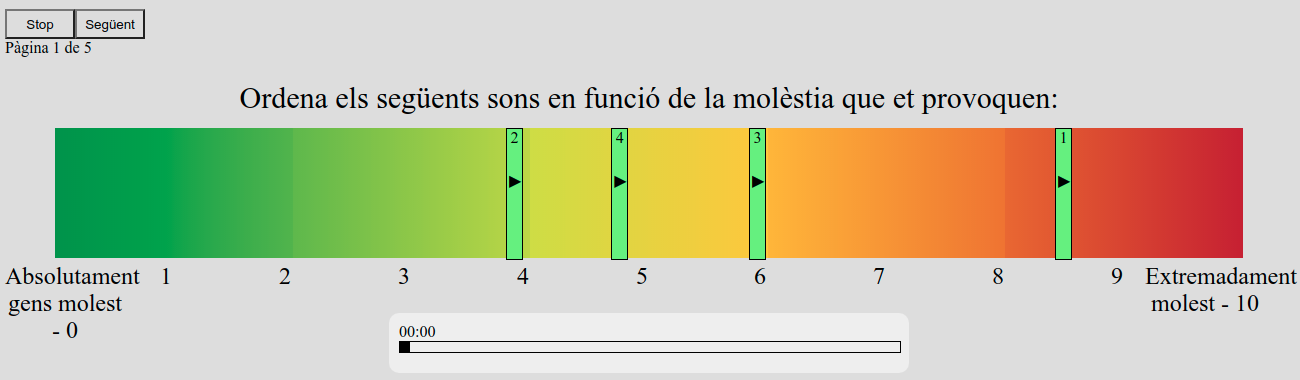
\includegraphics[width=\textwidth]{Figures/mushraScreenShot02.png}
  \caption{Screenshot of the \gls{mushra} test conducted to assess the annoyance provoked by different sounds. Title: sort the following sounds according to the cause annoyance. The scale ranges from \emph{not annoying at all} to \emph{extremely annoying}.}
\end{figure}

\subsection{Psychoacoustic Data Analysis}

The dataset resulted in 27 audio recordings of identified sound events with durations ranging between 1.01 and 2.69 s. The calibrated audio files were imported into the ArtemiS Suite software (v. 11.5, Head Acoustics GmbH) and the following psychoacoustic parameters were computed: \emph{loudness, sharpness, roughness, tonality} and \emph{impulsiveness} \citep{PsychoacousticsfactsmodelsZwicker}; values for these parameters are reported in Table \ref{tab:sensor-stimuli}. The rationale for selecting a relatively large set of psychoacoustic metrics is that they are often used as indicators to predict perceptual constructs (such as annoyance) in perceptual studies, as shown in recent soundscape literature \citep{Aletta2016Soundscape,Aletta2017Dimensions}. Fluctuation Strength, which could otherwise be included in this list of psychoacoustic parameters, as in Zwicker's annoyance model, was not included as the length of the recordings are too short to obtain a valid value. Loudness was calculated according to the DIN 45631 / A1 standard for time-varying sounds, in a free-field \citep{DIN2008Calculation}. As recommended by the standard, in order to avoid the under-estimation of evaluated loudness which is seen when using the arithmetic average of the loudness curve, the \gls{n5} value (the 5\% percentile value of the time-dependent loudness curve) is used as the single value of loudness. Sharpness was calculated according to \citet{DIN2009measurement}, in a free-field. With this sharpness method, the absolute loudness of the sound is not accounted for, so there should not be a duplication of information across the loudness and sharpness metrics. Roughness was calculated according to the hearing model by \citet{Sottek2017Sound}, with the option to skip the first 0.5 s in order to not distort the single value. Impulsiveness was also calculated according to the hearing model by Sottek, with a 0.5 s skip interval. Finally, tonality was calculated according to \citet{ECMA742019Measurement}, which is based on the hearing model of Sottek, with a frequency range of 20 Hz to 20 kHz.


\begin{table}
\centering
\caption{Psychoacoustic parameters calculated for the 27 stimuli used in the listening experiment. \label{tab:sensor-stimuli}}
\resizebox{\linewidth}{!}{%
\begin{tabular}{ccccccc} 
\toprule
\multirow{2}{*}{\textbf{Sensor }} & \multirow{2}{*}{\textbf{Label }} & \multicolumn{5}{c}{\textbf{Psychoacoustic Parameters }} \\ 
\cline{3-7}
 &  & \begin{tabular}[c]{@{}c@{}}\textbf{Loudness}\\\textbf{($N_5$ sone)}\end{tabular} & \begin{tabular}[c]{@{}c@{}}\textbf{Sharpness}\\\textbf{(acum)}\end{tabular} & \begin{tabular}[c]{@{}c@{}}\textbf{Roughness}\\\textbf{(asper)}\end{tabular} & \begin{tabular}[c]{@{}c@{}}\textbf{Tonality}\\\textbf{(tuHMS)}\end{tabular} & \begin{tabular}[c]{@{}c@{}}\textbf{Impulsiveness}\\\textbf{(iu)}\end{tabular} \\ 
\hline
hb133 & peop & 15.1 & 1.46 & 0.032 & 0.204 & 0.270 \\
hb133 & door & 16.8 & 1.43 & 0.029 & 0.113 & 0.354 \\
hb133 & dog & 13.1 & 1.22 & 0.033 & 0.373 & 0.266 \\
hb133 & brak & 16.0 & 1.76 & 0.030 & 0.326 & 0.241 \\
hb133 & bird & 12.6 & 1.73 & 0.024 & 0.283 & 0.214 \\
hb133 & airp & 13.0 & 1.27 & 0.060 & 0.438 & 0.231 \\ 
\hline
hb127 & sire & 17.7 & 1.56 & 0.045 & 1.540 & 0.178 \\
hb127 & peop & 16.1 & 1.62 & 0.035 & 0.410 & 0.417 \\
hb127 & horn & 18.1 & 1.56 & 0.028 & 0.666 & 0.260 \\
hb127 & door & 19.8 & 1.72 & 0.037 & 0.037 & 0.479 \\
hb127 & brak & 19.0 & 1.95 & 0.034 & 0.251 & 0.281 \\ 
\hline
hb127 & sire & 20.1 & 1.73 & 0.046 & 1.670 & 0.288 \\
hb127 & peop & 22.0 & 1.96 & 0.036 & 0.322 & 0.452 \\
hb127 & horn & 19.9 & 2.16 & 0.034 & 1.290 & 0.336 \\
hb127 & brak & 21.0 & 1.81 & 0.030 & 1.170 & 0.285 \\
hb127 & airp & 24.4 & 1.65 & 0.056 & 0.172 & 0.446 \\ 
\hline
hb115 & wrks & 20.3 & 1.97 & 0.054 & 0.227 & 0.267 \\
hb115 & trck & 24.4 & 1.60 & 0.033 & 0.040 & 0.276 \\
hb115 & sire & 19.5 & 1.46 & 0.054 & 0.861 & 0.333 \\
hb115 & peop & 25.1 & 1.79 & 0.032 & 0.411 & 0.331 \\
hb115 & horn & 22.3 & 2.00 & 0.032 & 0.806 & 0.155 \\
hb115 & door & 26.3 & 1.62 & 0.038 & 0.045 & 0.397 \\
hb115 & brak & 20.6 & 1.93 & 0.034 & 0.216 & 0.313 \\ 
\hline
hb115 & wrks & 24.6 & 1.92 & 0.064 & 0.447 & 0.317 \\
hb115 & sire & 26.6 & 1.77 & 0.044 & 0.626 & 0.290 \\
hb115 & horn & 29.5 & 2.35 & 0.039 & 0.486 & 0.262 \\
hb115 & door & 31.3 & 1.88 & 0.048 & 0.223 & 0.402 \\
\bottomrule
\end{tabular}
}
\end{table}

\subsection{Multi-Level Linear Regression Modelling}

The analysis for this study utilises a \gls{mlm}, with a random intercept and a random slope, using backward step feature selection. \glspl{mlm} are commonly used in psychological research for repeated measures studies \citep{Quene2004multi,VolpertEsmond2021Using} and for applied prediction models \citep{Gelman2006Multilevel,Frees2006Multilevel}. \gls{mlm} allows for the incorporation of nested and non-nested groups effects within the structure of the model, where the coefficients and intercepts for the independent variables are allowed to vary across groups. For this study, the data are grouped into two non-nested sets to form a two-level model: by repeated measures per respondent (\emph{user}) and by sound type (\emph{label}). In order to take into account the repeated measures across participants, and to correct for the participant's mean annoyance level, the \emph{user} variable is included in the second-level as a random intercept. We then include the psychoacoustic features as label effects, with coefficients which are allowed to vary across the sound type labels. The psychoacoustic features are also included as fixed effects in the first level, which do not vary across either the user or label groups.

The initial model structure, as written in Wilkinson-Rogers notation \citep{Wilkinson1973Symbolic}, is thus:

\begin{equation}
  % \begin{split}
  \label{eqn:initMLMann}
      Annoyance \sim N_5 + R + S + T + I + (1 | user) + (1 + N_5 + R + S + T + I | label)
  % \end{split}
  \end{equation}

\subsubsection{Feature Selection}

The \gls{mlm} is initially fitted with all of the potential features included within both levels. In order to reduce the complexity of the model, a backwards step features selection process is applied to both levels of the model. This process involves fitting the full model which includes all of the potential independent features (i.e. \cref{eqn:initMLMann}). The feature with the highest \emph{p}-value (least significant) is then removed from the candidates and the model is refit. This process is repeated until all features meet the predefined significance threshold of $p < 0.05 $. For a two-level model, first backward elimination of the second level is performed, followed by backward elimination of the first-level (or fixed) part.

If more than one feature is selected in the first-level, then the \gls{vif} is calculated in order to check for multicollinearity, with a pre-determined threshold of ${VIF}<5$. Any features which remain after the backwards stepwise selection and exceeded this threshold were investigated and removed if they were highly collinear with the other features. Once the feature selection process is completed, the final model with only significant features of interest included is fit and the table of the model coefficients is printed along with plots of the random effects and standardised estimates terms. Finally, quantile plots of the residuals and random effects are examined to confirm they are normally distributed \citep{Harrison2018brief}.

The input and output features are z-scaled prior to the analysis and model building by subtracting the mean and dividing by the standard deviation in order to directly compare the coefficient values of independent variables measured on different scales \citep{Harrison2018brief}. The model fitting and feature selection was performed using the \texttt{step} function from \texttt{lmerTest} (v. 3.1.3) \citep{Kuznetsova2017lmerTest} in the R statistical software (v. 4.0.5) \citep{RCT2018R}. The summaries and plots were created using the \texttt{sjPlot} package (v. 2.8.7) \citep{Luedecke2021sjPlot} and the multi-level $R^2$ values were calculated using \texttt{MuMIn} (v. 1.43.17) \citep{Barton2020MuMIN}.

%%%%%%%%%%%%%%%%%%%%%%%%%%%%%%%%%%%%%%%%%%%%%%%%%%%%%%%%%%%%%%%%%%%%%%%%%%%%%%%%

\section{Results}

\subsection{Differences in Annoyance between Groups \label{sec:groupDiffs}}
%NOTE: May remove this, it's Francesco's work

\footnote{The analysis carried out in \cref{sec:groupDiffs} was performed by Dr. Francesco Aletta. These results are included here verbatim from the original published paper to provide context for the later discussion on the influence of demographic differences on soundscape perception.}The average annoyance score of all users across all stimuli was $M=0.58 (SD=0.05)$. Since some basic demographic information about the 100 participants of the perceptual test was known, it seemed logical to explore possible differences in annoyance scores between different groups/levels of stratification of the sample, mostly for descriptive purposes. Therefore, Areas of residence and Gender were considered as factors in this analysis. Gender was treated as a binary variable (F/M), while Areas of residence was treated as a five-level categorical variable based on people's self-reported character of the area where they typically reside (range: 1-5; very quiet-very noisy). One-way repeated measures \gls{anova} was deemed to be the most appropriate approach to take into account the multiple responses that each of the 100 participants provided for the different recordings ($N=27$). A first analysis was then conducted to determine whether there was a statistically significant difference in annoyance between Areas of residence: no statistically significant differences were observed in this case $F(4.95)=1.374, p=0.249$. Likewise, a second one-way repeated measures \gls{anova} was carried out to check whether statistically significant differences in annoyance existed between females and males: no statistically significant effect was observed in this case either $F(1.98)=0.714, p=0.400$. Such small differences between groups can indeed be observed in Figure \ref{fig:anova}.

\begin{figure}[h]
  \label{fig:anova}
  \centering
  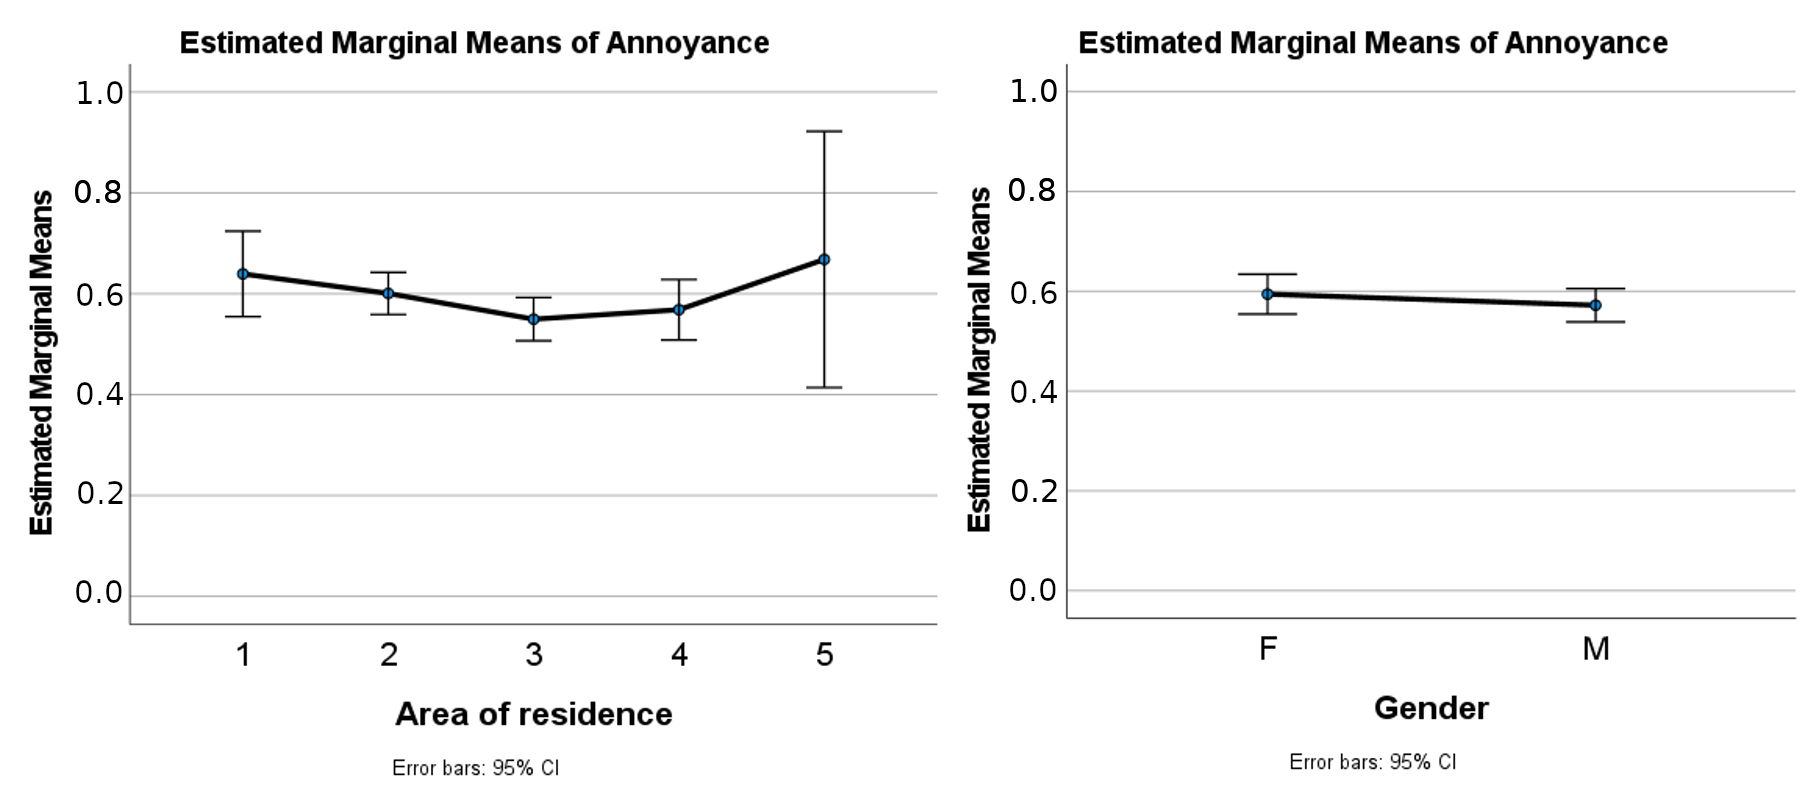
\includegraphics[width=\textwidth]{Figures/orga_anovas.png}
  \caption{Estimated Marginal Means for Annoyance as a function of Areas of residence (\textbf{left}) and Gender (\textbf{right}).}
\end{figure}

\subsection{Annoyance Model}
%TODO: Need to fix the ways I refer to the psychoacoustic features throughout the thesis. needs to be consistent
In the context of the multi-level linear regression modelling, the included variables were assumed to have an effect at two levels: the first level (i.e. fixed effect(s)), and the second level, where annoyance score intercepts are allowed to vary as a function of users (i.e. the 100 participants), and where each feature of interest is allowed its own coefficient as a function of labels (i.e. the 7 types of sounds). Sharpness came up as the main predictor with a strong statistical significance in the fixed-effect level, as reported in Table \ref{tab:annoyance-model}. This implies that, regardless of any other factors, the sharper the sounds, the more annoying they are perceived to be.

\begin{table}[h]
  \centering
  \caption{Random-intercept random-slope multi-level model of psychaocoustic annoyance, accounting for repeated measures (user) and sound source type (label) within the second level. Coefficients and confidence intervals given are for z-scaled data.}
  \label{tab:annoyance-model}
  \begin{tabular}{cccc} 
  \toprule
   & \multicolumn{3}{c}{\textbf{Annoyance }} \\ 
  \hline
  \textit{Predictors} & \textit{Estimates} & \textit{CI} & \textit{p} \\ 
  \hline
  (Intercept) & 0.02 & -0.13 -- 0.16 & 0.811 \\
  Sharpness & 0.33 & 0.25 -- 0.40 & \textbf{\textless{}0.001} \\ 
  \hline
  \textbf{Random Effects} &  &  &  \\ 
  \hline
  $\sigma^2$ & 0.47 &  &  \\
  $\tau_{00user}$ & 0.28 &  &  \\
  $\tau_{00label}$ & 0.02 &  &  \\
  ICC & 0.39 &  &  \\
  $N_{user}$ & 100 &  &  \\
  $N_{label}$ & 10 &  &  \\ 
  \hline
  Observations & 2700 &  &  \\
  Marginal $R^2$ / Conditional $R^2$ & 0.08 / 0.64 &  &  \\
  \bottomrule
  \end{tabular}
  \end{table}

The second-level effects presented in Figure \ref{fig:annoyance-effects} show that level- and loudness-based acoustic parameters do not play a significant role in predicting annoyance when considering other psychoacoustic factors and specific sound sources. However it should be noted that this may be influenced by the online data collection paradigm used in this study, which may struggle to control for the playback level. The variables selected by the feature selection algorithm within the type of sound (\emph{label}) level include: impulsiveness, roughness, tonality, and type of sound are relatively small, while roughness appears to be more important. For instance, when other effects are controlled, the sound type `horn' seems to be less annoying the rougher it is; while for the types of sound `bird' and `siren', higher roughness values will lead to higher annoyance scores. Looking at the model from the point of view of the types of sound, one could observe that `horns' tend to be more annoying than other sounds if they are more impulsive, while `people' or `birds' or `brakes' result in more annoying scores compared to other sounds if their tonal components are more prominent. Overall, for this model, the marginal and conditional $R^2$ values are 0.08 and 0.64, respectively. Marginal $R^2$ provides the variance explained by the fixed effects only, and conditional $R^2$ provides the variance explained by the whole model, i.e. both fixed effects and second-level effects. Thus, the majority of variance is explained by second-level factors, while a smaller portion (8\%) is covered by sharpness alone.

\begin{figure}[h]
  \label{fig:annoyance-effects}
  \centering
  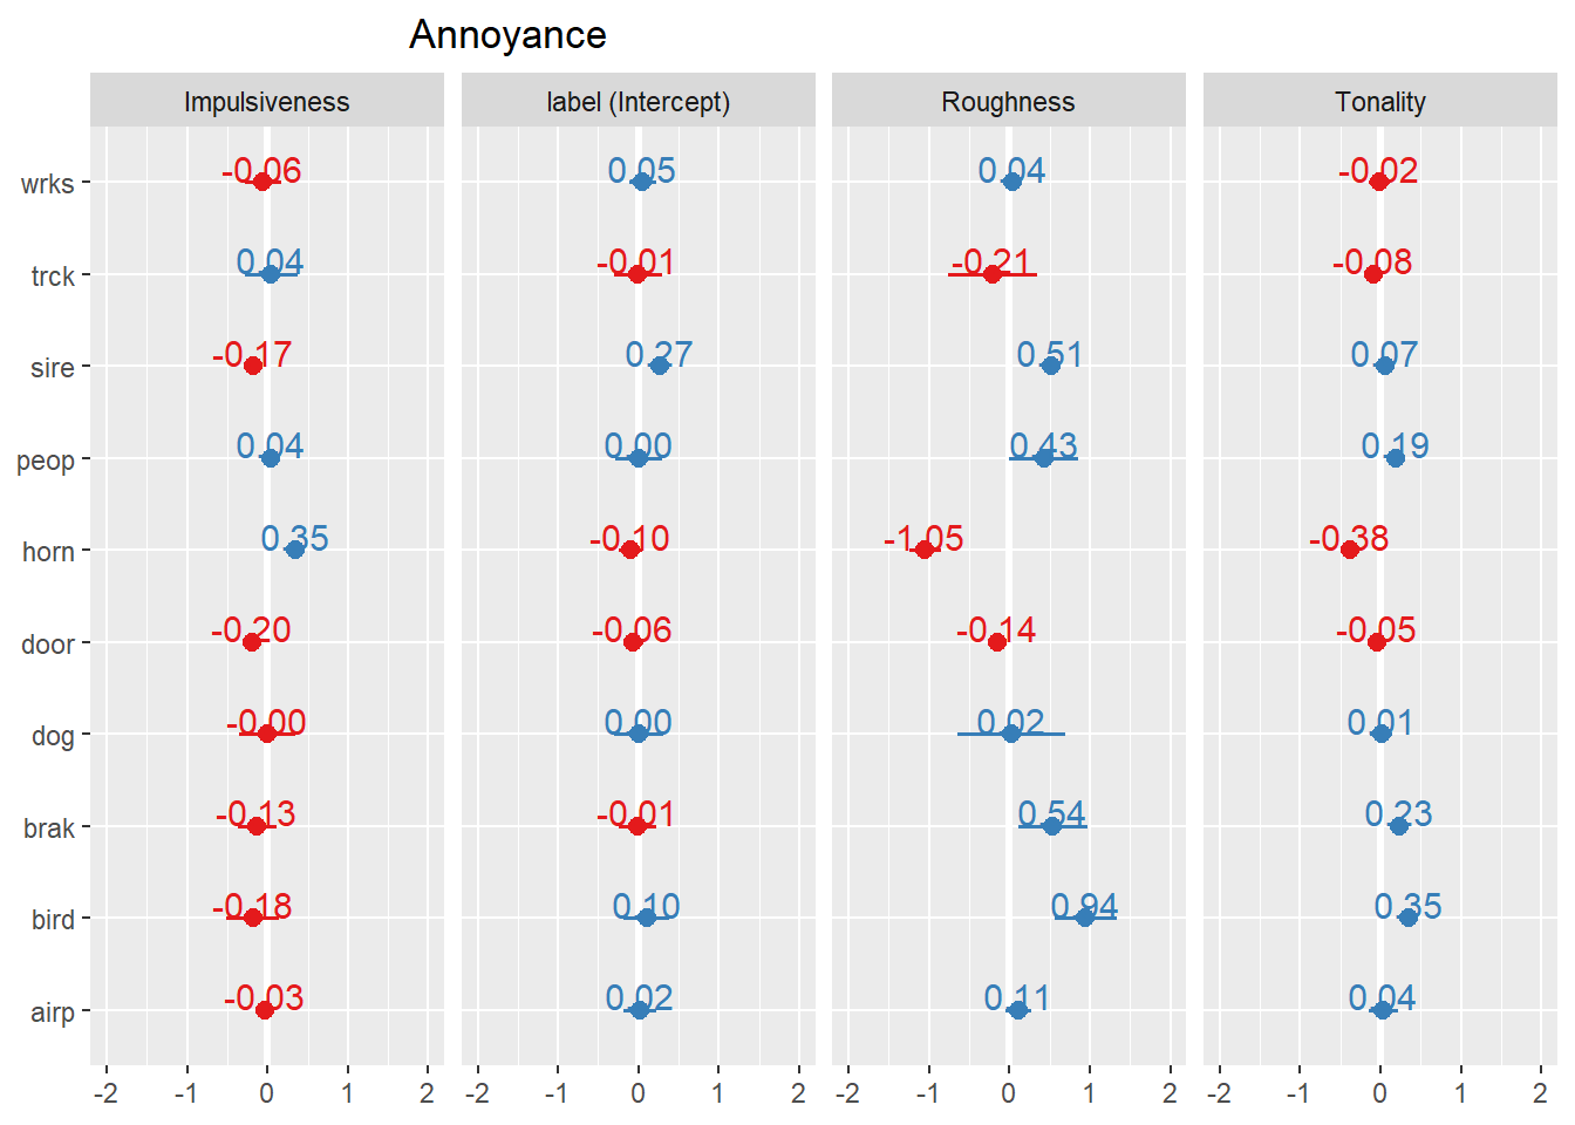
\includegraphics[width=\textwidth]{Figures/OrganMLMAnnoyanceRandom.png}
  \caption{Second-level effects figures representing the regression coefficients by types of sound (label) and for different psychoacoustic parameters.}
\end{figure}

%%%%%%%%%%%%%%%%%%%%%%%%%%%%%%%%%%%%%%%%%%%%%%%%%%%%%%%%%%%%%%%%%%%%%%%%%%%%%%%%%%%%%%%

\section{Discussion}

The fact that no significant differences in annoyance scores were observed between sample groups (i.e. gender or area of residence) is particularly interesting: it is common to assume in soundscape studies that personal and contextual factors play a strong role in how people respond to urban acoustic environments \citep{Kang2016Ten}. However, this is probably more relevant when complex sound environments (e.g. multi-source) are being considered and when dealing with relatively longer duration of exposures (e.g. several minutes) as seen in in-situ surveys. For clearly identifiable sources of environmental noise, with signals of short duration (i.e. 1-3s) like those used for this experiment, it is likely it was easier for the sample to converge on similar annoyance scores, regardless of other demographic factors. This aspect will be further investigated in \cref{ch:whostudy}.

Regarding the noise annoyance scores, sharpness came up as an important predictor in the first level of the modelling stage (explaining up to 8\% of the variance alone). It is important to highlight that the sharpness calculation method used in this study did not include any loudness correction; nor was any loudness-related parameter selected by the feature selection algorithm. To some extent, this is possibly due to the fact that, being an online experiment, it was not possible for the research team to actually calibrate the loudness playback level accurately for the remote participants. On the other hand, considering this aspect from the \gls{wasn} implementation perspective, this could be seen as an encouraging finding, since calibrating a diffuse acoustic monitoring network may not be practical in real-world scenarios, so it is good to have models that can achieve up to 64\% of variance explained regardless of actual levels. Furthermore, in complex acoustic environments, loudness would likely vary over time depending on the relative positions between sound sources and (human) listeners in ways in which the other psychoacoustic parameters such as sharpness and tonality are less likely to. This is something that is impossible for fixed sensors to take into account, so once again it is preferable not to rely on loudness as a predictor.

This result also appears to differ from some of the results in the model from \cref{ch:lockdown}, where sharpness was not selected as a final feature in the \gls{isopl} model. There are a few potential explanations for this. First, although within the circumplex pleasantness is considered the opposite of annoying, the respondents' annoyance rating in this study may be focussed on more specific or different factors than what is captured in the combined \gls{isopl} score. Second, since the \gls{isd} data is collected \emph{in-situ}, the general pleasantness of the soundscape may emphasise different acoustic features than the online study procedure used in this study. Finally, the structure of this model effectively controls for the influence of sound source information, whereas the \cref{ch:lockdown} model has no source information included. This could be interpreted as the sound-source-aware model more correctly identifying the acoustic feature which is important, independent of the sound source. Whereas the previous model's feature selection results may be more likely to select the features which help to differentiate sound sources, that is not necessary in the sound-source-aware model. This would indicate that the features selected in the \cref{ch:lockdown} model were selected because they perform better at differentiating sound sources and accounting for the semantic meaning associated with sound sources, but when the semantic information itself is included in the model, other acoustic features are more important for determining annoyance. 

Being able to predict noise annoyance from recorded sounds is particularly helpful from a public health perspective. In the context of a smart-city framework, one could imagine a \gls{wasn} large enough to cover a whole urban area; having a noise annoyance prediction algorithm at the node position that can return live annoyance scores to a central server from sounds recorded locally by the sensor would make for a useful application for environmental protection officers and other stakeholders at community or local authority level \citep{Kang2018Impact}. A relevant issue to consider from the \gls{wasn} perspective, is that in previous studies conducted in both urban \citep{Alias2020WASN} and \citep{Alias2020Aggregate} environments, a clear influence of the type of environment around the sensor location on the types of noise was seen. Not all urban and suburban locations around the sensors have frequent sirens or horns. The presence of these sounds depends on the most common activities (e.g. leisure, hospitals, etc.), the type of road (wide, narrow), and the type of buildings and houses surrounding the location. The types of sounds and their relative frequency of occurence can vary widely given the combination of these architectural and landscape characteristics. In the design of a general model for quality of life, the approach for considering sound source information presented in this chapter should be combined with the proposal for incorporating this architectural and contextual information developed previously in \cref{ch:bayes}.

% \subsection*{Positivity (or the absence of negativity?)}
% \draft{NEW!!}
% From the experience of the previous studies which are highly focused on the existing environmental acoustic and psychoacoustic metrics, one (of many) potential limitations has been revealed. For the most part, these metrics were designed to characterise various negative qualities of the sound. Certainly, they therefore have a negative correlation with positive assessments of the sound, but the simple fact is that they were conceived of and implemented in an attempt to quantify some sonic characteristic that was assumed by the researchers to contribute to a negative perception. Hence why in Zwicker's empirical formula for Psychoacoustic Annoyance \citep{PsychoacousticsfactsmodelsZwicker} $PA = N_5 (1 + \sqrt{\omega^2_S + \omega^2_{FR}})$, all of the constituent parts have positive coefficients.

% While this would not theoretically hinder a formula for describing positive aspects of the sound, it creates a sort of conceptual barrier. If all of these metrics are designed to capture negative aspects of the sound, then it is insufficient to use them create a formula to describe a positive sound, since that formula would only represent the 'absence of negativity', not necessarily positivity.

%TODO: Add a more indepth discussion and add a limitation  section to lead into DeLTA

\subsection{Incorporating into the general model}
Incorporating information about the sound source can greatly improve the prediction of perceived annoyance. The modelling structure used in this chapter effectively created separate, sound-source-dependent models of psychoacoustic annoyance, in contrast to the general annoyance model developed by \citet{PsychoacousticsfactsmodelsZwicker}. Each sound source (traffic, horns, people, etc.) has its own linear combination of psychoacoustic values to demonstrate how the semantic meaning which the listener assigns to a sound mitigates the perceptual mapping from physical inputs to perceptual outcomes. Incorporating this information, such that this semantic meaning influences the outcome of the ideal predictive model, is crucial. What is less clear is 1) how to deal with complex scenes where multiple overlapping sound sources are present and how to integrate this into the model; and 2) how this process can be automated, with minimal manual input from the model's users. %TODO: Expand on sound source inclusion

Given the somewhat unexpected result from this study that demographic factors had little difference on annoyance ratings, the next chapter will further investigate the influence of personal factors on soundscape perception making use of the larger and more diverse dataset from the \gls{isd}.


%%%%%%%%%%%%%%%%%%%%%%%%%%%%%%%%%%%%%%%%%%%%%%%%%%%%%%%%%%%%%%%%%%%%%%%%%%%%%%%%%%%%%

%DONE: Restructure the Conclusion and Incorporating sections to be more cohesive with the rest of Part C
\section{Conclusions}

In this chapter, an online listening experiment was conducted with 100 participants to assess the noise annoyance induced by short recordings of individual environmental noise sources gathered via a wireless acoustic sensors network in Milan. The main conclusions of this study are:

\begin{itemize}
  \item The acoustic samples gathered from selected sensors in Milan \gls{wasn} of the DYNAMAP project led the DYNAMAP team to a structured \gls{mushra} test to evaluate the annoyance in an offline perceptual test.
  \item When considering short recordings of single-source environmental sounds, no significant differences in noise annoyance were observed as a function of demographic factors, such as gender and self-reported area of residence (i.e. from very quiet to very noisy).
  \item The multi-level linear regression model derived from this case study achieved an overall $R^2=0.64$, using sharpness as a fixed effect (the first level), and impulsiveness, roughness, and tonality as random effects allowed to vary according to the type of sound (the second level) as predictors for perceived noise annoyance.
\end{itemize}

%DONE: need ot rephrase this
% Taken together, the results of this study encourage us to continue our research work at all the stages described in this paper. The improvement of real-time algorithms to automatically detect the predefined sound sources under study is the first stage to gathering the most relevant samples in all and each of the sensors of a \gls{wasn}. The application of the annoyance modelling can give the \gls{wasn} a dimension without precedent: the availability of the objective acoustic measurements conducted by the sensors, and the estimation of annoyance in a real-time evaluation by means of the model. We can start to think about a dynamic annoyance map, which could be more far-reaching than a dynamic noise map.

